\chapter{Étude préalable, architecture et environnement technique}
\label{ch:architecture}
\startcontents[chapters]
\chapterplan

\section{Introduction}

L'analyse des besoins a défini les fonctions attendues de SEPAPaie et les responsabilités de ses utilisateurs. Leur réalisation nécessite désormais de relier les exigences métier aux choix de conception. Ce chapitre présente les notions essentielles du domaine SEPA, puis justifie l'association de règles explicites et d'une détection d'anomalies par apprentissage non supervisé. Il décrit ensuite l'architecture retenue, les échanges entre ses composants et l'environnement technique utilisé. L'objectif est d'expliquer les choix structurants du projet, sans anticiper les détails de réalisation ni les résultats d'évaluation présentés dans les chapitres suivants.

\section{Étude du domaine métier}

\subsection{Le virement SEPA appliqué à la paie}

Le \textbf{SEPA}, ou espace unique de paiements en euros, vise à harmoniser les paiements en euros entre les pays participants. Il ne se limite donc pas aux seuls pays de la zone euro. Le schéma de virement SEPA, appelé \textit{SEPA Credit Transfer} (SCT), définit des règles communes pour les virements nationaux et transfrontaliers. Il permet notamment de préparer des paiements groupés, tels que les virements mensuels de salaires~\cite{epc-sct}.

Dans ce contexte, une société est le \textbf{débiteur} : son compte est débité du montant des rémunérations. Les salariés sont les \textbf{bénéficiaires} des virements. Un lot rassemble plusieurs instructions individuelles, associées à une date d'exécution et aux coordonnées bancaires de la société. Cette organisation explique le choix de SEPAPaie de préparer un fichier pour une seule société débitrice, tout en regroupant plusieurs salariés.

Le projet s'inscrit dans le contexte de la paie HR Access, mais la réalisation présentée est une plateforme autonome de préparation et de contrôle des données de paiement. Elle ne constitue ni un moteur de calcul de la paie ni un connecteur de production déjà raccordé à HR Access. Elle ne réalise pas non plus le transfert bancaire : son périmètre s'arrête à la préparation, au contrôle, à la validation interne et au téléchargement du fichier.

\subsection{ISO 20022 et le message \texttt{pain.001}}

\textbf{ISO~20022} fournit un cadre de définition des messages financiers. Il convient de distinguer ce standard du schéma SEPA : ISO~20022 décrit les messages, tandis que les règles et les guides d'implémentation SEPA précisent leur utilisation dans un contexte de paiement donné~\cite{iso20022,epc-guides}.

Pour l'initiation des virements, le message utilisé est \texttt{pain.001}, nommé \textit{Customer Credit Transfer Initiation}. Il représente les instructions adressées par un client à son prestataire de services de paiement. Dans sa représentation XML, il comprend une enveloppe \texttt{Document}, puis un élément \texttt{CstmrCdtTrfInitn}. Le tableau~\ref{tab:structure-pain} présente ses principaux blocs, sans détailler l'ensemble des balises du standard.

\begin{table}[H]
\centering
\small
\renewcommand{\arraystretch}{1.25}
\tablestyle
\begin{tabularx}{\textwidth}{|>{\raggedright\arraybackslash}p{3.5cm}|Y|Y|}
\hline
\rowcolor{appMarine}\entete{Bloc} & \entete{Rôle} & \entete{Exemples de données} \\
\hline
En-tête du groupe (\texttt{GrpHdr}) & Identifier le message et décrire le groupe de virements & Identifiant du message, date de création, nombre de transactions, somme de contrôle \\
\hline
Informations de paiement (\texttt{PmtInf}) & Définir les paramètres communs du lot & Société débitrice, compte à débiter, date d'exécution, méthode de paiement \\
\hline
Virement individuel (\texttt{CdtTrfTxInf}) & Décrire une instruction destinée à un bénéficiaire & Référence du virement, montant et devise, nom et IBAN du bénéficiaire, libellé \\
\hline
\end{tabularx}
\caption{Principaux blocs d'un message \texttt{pain.001}}
\label{tab:structure-pain}
\end{table}

Dans la plateforme, le nombre de transactions et la somme des montants sont calculés à partir des fiches sélectionnées. Le fichier porte également une référence de message et des références de virements. Ces informations permettent de rapprocher le contenu généré des données de préparation.

Plusieurs versions de \texttt{pain.001} existent. La réalisation prend notamment en compte les versions \texttt{pain.001.001.03} et \texttt{pain.001.001.09}, dont certaines structures diffèrent : le code bancaire est représenté par \texttt{BIC} dans la première et par \texttt{BICFI} dans la seconde ; la représentation de la date d'exécution évolue également. Le choix du schéma doit donc rester cohérent avec la version du document généré. Cette prise en compte ne signifie pas que toute version future ou toute variante bancaire est automatiquement supportée.

\subsection{Le rôle du schéma XSD}

Un schéma \textbf{XSD} décrit la structure et les contraintes d'un document XML : éléments autorisés, ordre d'apparition, champs obligatoires, types et restrictions de valeurs~\cite{w3c-xsd}. La validation XSD permet ainsi de repérer une balise absente, une structure incompatible ou une valeur qui ne respecte pas le type attendu.

SEPAPaie permet de gérer les schémas et de sélectionner celui qui convient à la génération. Le document produit est ensuite vérifié contre ce schéma. Les erreurs sont restituées sous une forme exploitable par l'utilisateur, afin qu'il puisse corriger les données ou revoir le schéma sélectionné.

Il faut toutefois distinguer \textbf{conformité de structure} et \textbf{exactitude métier}. Un salaire excessif, un compte bancaire appartenant à la mauvaise personne ou un paiement en double peuvent respecter le XSD. De même, la conformité à un schéma ne garantit pas à elle seule l'acceptation du fichier par une banque, qui peut appliquer des contraintes supplémentaires. C'est pourquoi la plateforme complète cette validation par des contrôles métier et une analyse des paiements.

\subsection{Les coordonnées bancaires : IBAN et BIC}

L'\textbf{IBAN} identifie un compte bancaire. Il comprend un code pays, deux chiffres de contrôle et une partie nationale dont la structure dépend du pays. Le contrôle de la clé repose sur un calcul modulo~97 : après déplacement des quatre premiers caractères à la fin et conversion des lettres en valeurs numériques, le reste attendu est égal à~1.

La plateforme utilise ce contrôle pour signaler les IBAN incohérents. Il permet de détecter de nombreuses erreurs de saisie, mais ne prouve ni l'existence du compte ni son appartenance au salarié. Une vérification auprès d'une source bancaire fiable reste donc nécessaire lorsqu'une anomalie porte sur le bénéficiaire.

Le \textbf{BIC} identifie un établissement ou une entité dans les échanges financiers. Son format comporte huit caractères, éventuellement complétés par trois caractères identifiant une branche. Dans SEPAPaie, le format du BIC est contrôlé lorsqu'il est renseigné. Son absence et son caractère obligatoire sont à apprécier selon le schéma et le contexte de paiement ; il ne doit pas être présenté comme systématiquement obligatoire pour tout virement SEPA. Là encore, une vérification de format ne constitue pas une consultation d'un annuaire bancaire.

\section{Choix d'une détection hybride des anomalies}

\subsection{Apport et limites des règles métier}

Les règles métier traduisent des exigences connues en conditions vérifiables. Elles conviennent aux incohérences explicites : montant nul ou négatif, IBAN invalide, BIC mal formé ou répétition potentielle d'un paiement. Leur intérêt tient à leur lisibilité : l'utilisateur comprend directement la cause du signalement et l'action attendue.

Cependant, ces règles couvrent essentiellement les situations anticipées. Un montant positif peut être techniquement correct mais inhabituel pour le salarié concerné. Un seuil uniforme peut également produire trop d'alertes pour certains profils et manquer des variations significatives pour d'autres. La détection doit donc tenir compte du contexte, sans remplacer les règles qui restent nécessaires.

\subsection{Intérêt de l'apprentissage non supervisé}

Une approche supervisée suppose de disposer d'exemples suffisamment nombreux et fiables de paiements normaux et anormaux. Or le projet ne dispose pas d'un historique de paie de production accompagné d'anomalies confirmées. Les données synthétiques permettent de développer et d'évaluer la solution, mais ne remplacent pas cette connaissance du terrain.

L'\textbf{apprentissage non supervisé} constitue un point de départ pertinent : il recherche des observations atypiques sans exiger d'étiquette pour chaque exemple d'entraînement. Dans notre cas, un paiement est décrit par des variables telles que son montant, son écart par rapport à l'historique disponible, sa variation par rapport au paiement précédent ou un changement d'IBAN. Les détails de ces variables et de leur préparation sont présentés au chapitre~\ref{ch:sprint4}.

Le modèle choisi est \textbf{Isolation Forest}~\cite{liu2008isolation}. Son principe consiste à isoler les observations par des partitions aléatoires successives. Les observations atypiques tendent à être isolées plus rapidement que celles situées dans les régions les plus denses des données~\cite{sklearn-iforest}. Ce fonctionnement se prête à l'analyse de variables numériques décrivant les paiements et bénéficie d'une implémentation disponible dans scikit-learn.

Ce choix ne signifie pas qu'Isolation Forest est nécessairement le meilleur modèle pour toute population salariale. Il constitue le modèle intégré à la plateforme ; sa pertinence est étudiée expérimentalement, avec d'autres approches, au chapitre~\ref{ch:sprint4}. Un score élevé indique un caractère inhabituel, et non une probabilité démontrée de fraude.

\subsection{Complémentarité des contrôles}

L'approche retenue réunit trois niveaux complémentaires : validation de la structure XML, règles métier et détection des profils atypiques. Le tableau~\ref{tab:controle-hybride} précise leur portée.

\begin{table}[H]
\centering
\small
\renewcommand{\arraystretch}{1.25}
\tablestyle
\begin{tabularx}{\textwidth}{|>{\raggedright\arraybackslash}p{2.7cm}|Y|Y|}
\hline
\rowcolor{appMarine}\entete{Niveau} & \entete{Question traitée} & \entete{Limite principale} \\
\hline
Validation XSD & Le document respecte-t-il la structure et les contraintes du schéma sélectionné ? & Ne vérifie pas que le salaire ou le bénéficiaire est correct dans le contexte métier \\
\hline
Règles métier & Les données respectent-elles les conditions explicites de préparation du paiement ? & Ne couvrent pas toutes les situations inhabituelles \\
\hline
Analyse par IA & Le profil de paiement présente-t-il des caractéristiques atypiques ? & Peut produire des faux positifs et manquer certaines anomalies \\
\hline
\end{tabularx}
\caption{Complémentarité des niveaux de contrôle}
\label{tab:controle-hybride}
\end{table}

La décision du service Python combine le modèle statistique et une règle complémentaire portant sur le changement d'IBAN. L'analyse dite \og IA\fg{} n'est donc pas exclusivement statistique. Les explications et les recommandations sont également construites à partir de critères explicites appliqués aux variables du paiement ; elles ne sont pas générées par un modèle de langage.

Les anomalies métier bloquantes et les avertissements doivent rester distincts. Un signalement de montant suspect est une invitation à vérifier la fiche, et non un rejet automatique. De plus, la désactivation ou l'indisponibilité de la détection des montants ne doit pas interrompre les contrôles métier et XSD ; cette situation est indiquée dans le résultat.

Enfin, la décision humaine conserve son propre rôle. L'\textbf{approbation d'une fiche} porte sur un paiement individuel. Les contrôles du virement de masse portent sur une sélection, son contenu et le document produit. La \textbf{validation du fichier par le Manager} constitue ensuite une décision sur le lot soumis. Ces étapes ne se confondent pas : elles répondent à des questions différentes et assurent une vérification à plusieurs niveaux.

\section{Architecture de la solution}

\subsection{Vue d'ensemble et principes retenus}

SEPAPaie repose sur une \textbf{architecture web client--serveur}, organisée autour d'un backend central. Celui-ci regroupe les fonctions métier et expose une API consommée par l'interface. Les traitements Python sont placés dans un service distinct. Cette organisation correspond à un backend métier modulaire accompagné d'un service spécialisé, et non à une architecture de microservices pour chaque fonction.

La figure~\ref{fig:architecture-logique} présente les responsabilités et les principales dépendances. La banque et HR Access ne sont pas représentés comme des services connectés, car aucun échange de production avec ces systèmes n'est réalisé dans le périmètre présenté.

\begin{figure}[H]
\centering
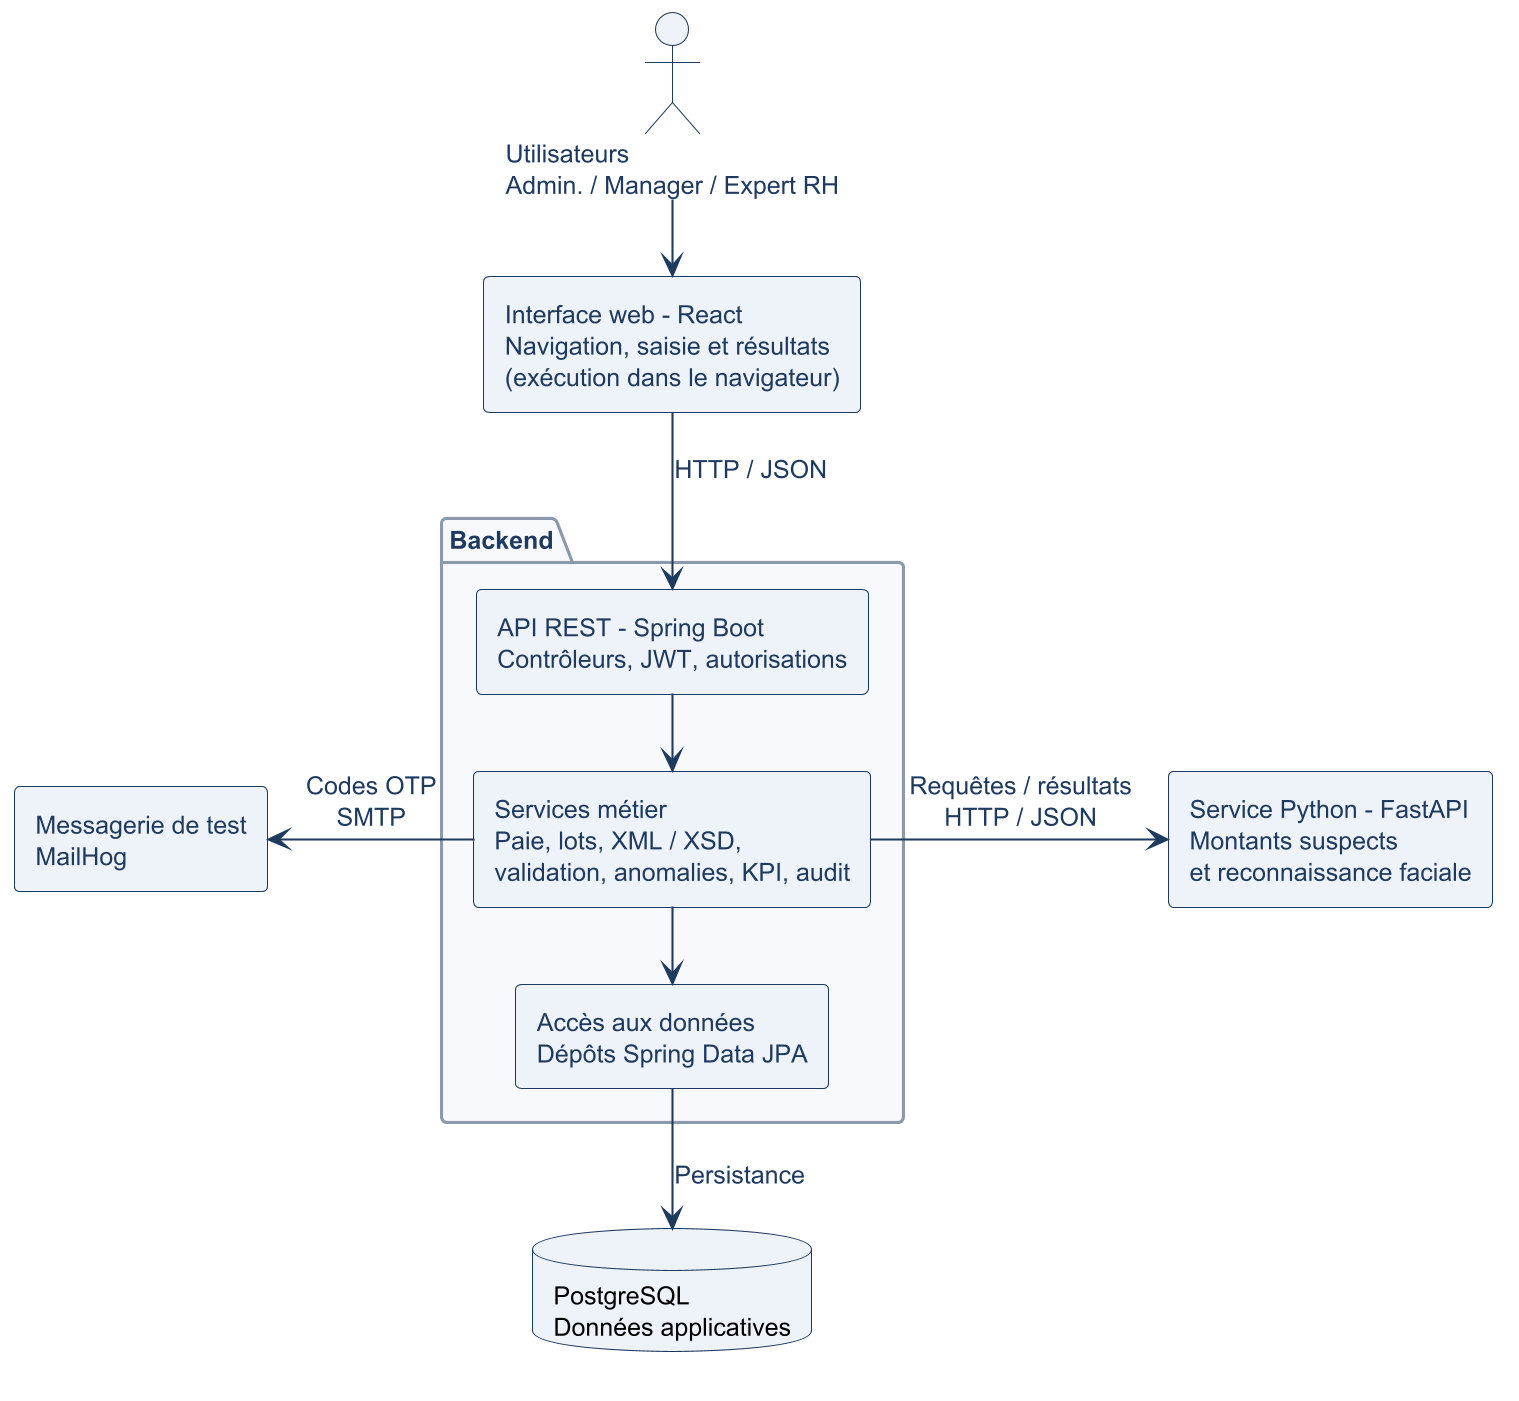
\includegraphics[width=\textwidth,height=0.60\textheight,keepaspectratio]{fig3_1_architecture_logique}
\caption{Architecture logique de SEPAPaie}
\label{fig:architecture-logique}
\end{figure}

L'\textbf{interface React} assure la navigation, la saisie et la restitution des résultats. Le \textbf{backend Spring Boot} contrôle les accès, applique les règles et orchestre la préparation des fichiers. \textbf{PostgreSQL} conserve les données applicatives. Le \textbf{service FastAPI} prend en charge la détection des montants suspects et les traitements de reconnaissance faciale. Enfin, \textbf{MailHog} représente la messagerie de test utilisée pour recevoir les codes à usage unique.

Le backend constitue le point d'entrée des opérations métier. Le fait de masquer une action dans l'interface ne suffit pas à l'autoriser ou à l'interdire : la décision d'accès appartient au serveur. Cette centralisation évite de disperser les règles de validation.

\subsection{Organisation logicielle en couches}

Le backend est organisé selon une séparation des responsabilités :
\begin{itemize}
    \item la \textbf{couche API} reçoit les requêtes HTTP et retourne des réponses adaptées à l'interface, à travers des contrôleurs et des objets de transfert ;
    \item la \textbf{couche de services} porte les règles métier et les enchaînements : préparation des lots, génération XML, contrôles, soumission, validation, recommandations et indicateurs ;
    \item la \textbf{couche d'accès aux données} utilise les dépôts Spring Data JPA pour lire et enregistrer les entités dans PostgreSQL ;
    \item les \textbf{composants transversaux} assurent notamment l'authentification, les autorisations, l'audit, la messagerie et les appels au service Python.
\end{itemize}

Cette séparation facilite les tests et limite le couplage : la génération XML peut être vérifiée indépendamment de l'interface, et le client HTTP du service Python peut être remplacé par un substitut dans les tests du backend.

\subsection{Circulation des données}

Lors d'un contrôle de virement de masse, les échanges suivent le parcours général ci-dessous :
\begin{enumerate}
    \item L'Expert RH sélectionne une société, une période et des fiches approuvées dans l'interface.
    \item Le navigateur transmet la demande au backend. Celui-ci vérifie l'accès à la société et charge les paiements sélectionnés.
    \item Si l'analyse des montants est activée, le backend prépare une requête contenant les paiements et leur historique disponible, puis l'envoie au service Python.
    \item Le service calcule les variables et retourne, pour chaque paiement, un score, un signalement éventuel et les éléments d'explication associés.
    \item Le backend exécute les contrôles métier, construit le XML et vérifie sa conformité au XSD. Il conserve le résultat et les informations utiles à la traçabilité.
    \item L'interface affiche la synthèse, les contrôles métier, l'analyse IA, la conformité XSD et l'aperçu XML.
\end{enumerate}

Le service Python \textbf{ne consulte pas directement PostgreSQL}. Les données nécessaires lui sont transmises par le backend sous forme de messages JSON. Il n'assure pas non plus la génération du fichier SEPA ni sa validation par le Manager.

Dans le parcours complet de contrôle, un résultat non conforme au XSD peut être conservé avec le statut \og Non conforme\fg{}, afin que ses erreurs restent consultables. Cet enregistrement ne vaut pas autorisation de téléchargement ni validation du fichier. Les conditions de soumission et de décision du Manager sont détaillées au chapitre~\ref{ch:sprint3}.

\subsection{Authentification et dépendances de sécurité}

Les appels protégés de l'interface vers le backend utilisent un jeton \textbf{JWT}. Spring Security vérifie l'authentification et les autorisations associées aux opérations. Les mots de passe sont conservés sous forme hachée ; les données XML sont traitées avec des restrictions d'accès aux ressources externes.

Deux parcours de connexion sont proposés : mot de passe suivi d'un code envoyé par courriel, ou reconnaissance faciale. Dans le premier, le backend dialogue avec la messagerie. Dans le second, il sollicite les traitements de visage du service Python, qui utilisent OpenCV.

Il convient de distinguer ces deux usages du service Python. L'analyse des montants est conçue comme une aide non bloquante pour le contrôle des fichiers. En revanche, une indisponibilité du traitement facial empêche le parcours de connexion par le visage ; elle ne doit pas être interprétée comme une réussite d'authentification. Le parcours par mot de passe et code conserve ses propres dépendances.

\section{Choix technologiques}

Les choix privilégient l'adéquation aux traitements, la séparation des responsabilités et la disponibilité d'outils de test. React répond aux besoins d'interaction et d'adaptation aux profils, Java structure les traitements métier et Python permet d'utiliser directement les bibliothèques d'apprentissage et de vision. Une réalisation dans un seul environnement aurait limité l'accès à l'écosystème Python, tandis qu'une multiplication de microservices aurait accru la complexité sans nécessité. Le backend central et le service spécialisé constituent un compromis, au prix d'une dépendance réseau dont les indisponibilités doivent être gérées. Le tableau~\ref{tab:technologies} synthétise les technologies principales.

\begin{table}[H]
\centering
\small
\renewcommand{\arraystretch}{1.25}
\tablestyle
\begin{tabularx}{\textwidth}{|>{\raggedright\arraybackslash}p{3.7cm}|Y|}
\hline
\rowcolor{appMarine}\entete{Technologie} & \entete{Rôle et justification} \\
\hline
React 18, Vite et Ant Design & Interface web organisée en composants ; outils de construction et composants graphiques pour les formulaires, tableaux et étapes du parcours \\
\hline
Java 17 et Spring Boot 3 & API métier, orchestration des contrôles, génération XML et intégration des services ; environnement adapté aux applications structurées \\
\hline
Spring Security et JWT & Authentification des requêtes et contrôle des autorisations côté serveur \\
\hline
Spring Data JPA et PostgreSQL 16 & Accès aux données et stockage relationnel des utilisateurs, référentiels, paiements, fichiers et traces \\
\hline
Python 3.11 et FastAPI & Service spécialisé avec contrats de requête et de réponse définis ; séparation des traitements Python du backend métier \\
\hline
scikit-learn, pandas et NumPy & Préparation des variables, entraînement et utilisation d'Isolation Forest, analyse des données d'évaluation \\
\hline
OpenCV & Détection du visage et comparaison de représentations faciales pour le parcours de connexion dédié \\
\hline
Docker Compose et MailHog & Exécution reproductible des services et réception locale des courriels de test \\
\hline
\end{tabularx}
\caption{Technologies principales de SEPAPaie}
\label{tab:technologies}
\end{table}

Ces technologies restent complémentaires : Spring Boot conserve les décisions métier, Python réalise les traitements spécialisés et Docker facilite la reproduction de l'environnement.

Le choix de \textbf{React} pour l'interface mérite une précision. Ce cadre, fondé sur une composition par composants réutilisables et un écosystème riche (notamment la bibliothèque de composants Ant Design, adaptée aux formulaires, tableaux et parcours en étapes de l'application), permet un prototypage rapide et des retours fréquents, en cohérence avec la démarche agile retenue. Associé à l'outil de construction Vite, il offre un cycle de développement court. Un autre cadre de même génération aurait également convenu ; React a été préféré pour sa simplicité de prise en main et la maturité de son écosystème au regard des besoins du projet.

\section{Environnement de développement}

Le développement est réalisé dans \textbf{Visual Studio Code}, avec \textbf{Git} pour le suivi des modifications, \textbf{Maven} et \textbf{npm} pour les dépendances du backend et de l'interface. Les tests du backend utilisent \textbf{JUnit} et les outils de test Spring Boot ; les traitements Python et le protocole d'évaluation sont vérifiés avec \textbf{pytest}. L'API est documentée de façon interactive par \textbf{OpenAPI et Swagger UI} (chapitre~\ref{ch:sprint5}). Enfin, \textbf{PlantUML} produit les diagrammes à partir de sources textuelles et \textbf{LaTeX} assure la mise en forme du rapport. Le déploiement par conteneurs et la recette de l'application complète sont présentés au chapitre~\ref{ch:sprint5}.

\section{Conclusion}

L'étude préalable met en évidence la nécessité de distinguer structure du fichier, cohérence des paiements et décision de validation. SEPA et ISO~20022 fournissent le cadre des échanges, tandis que les règles métier et l'analyse des profils atypiques complètent la conformité XSD. L'approche hybride retenue conserve l'utilisateur au centre de la décision.

L'architecture traduit ces principes en responsabilités séparées : React pour l'interaction, Spring Boot pour le métier, PostgreSQL pour la persistance et FastAPI pour les traitements spécialisés. L'environnement Docker Compose permet de reproduire la démonstration locale, sans être assimilé à un déploiement de production. Le chapitre suivant présente la réalisation du premier sprint, consacré au socle sécurisé et à l'administration.

